% 简谐振子

% 未完成:讲述太粗糙
\pentry{胡克定律, 牛顿第二定律\upref{New3}}

\begin{figure}[ht]
\centering
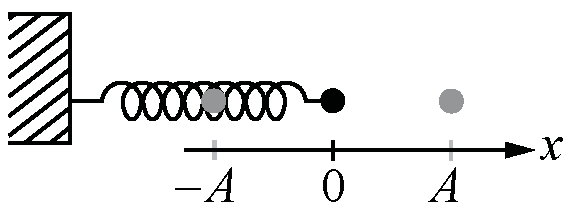
\includegraphics[width=6cm]{./figures/SHO.pdf}
\caption{简谐振子模型} \label{SHO_fig1}
\end{figure}

如\autoref{SHO_fig1}, 质量为 $m$ 的质点固定在弹性系数为 $k$ 的弹簧的一端,弹簧另一端固定.在 $t = 0$ 时,若质点不在平衡位置,或者有一个初速度,则接下来会发生振动(忽略弹簧的质量, 任何摩擦以及重力). 以质点拉伸弹簧的方向为 $x$ 轴正方向,质点的平衡位置为 $x = 0$. 当质点在位置 $x$ 时,根据胡克定律,受力为 $F =  - kx$. 根据牛顿第二定律\upref{New3} $F = ma = m\ddot x$ ( $\ddot x$ 代表对时间的二阶导数).  两式消去 $F$, 得
\begin{equation}\label{SHO_eq1}
m\ddot x =  - kx
\end{equation}
这是一个单变量函数与其二阶导数的关系式. 我们把这样含有单变量函数及其导数或高阶导数的等式叫做\bb{常微分方程}. 由于上式中最高阶导数是二阶,所以叫做\bb{二阶微分方程}. 要解该方程,就是要寻找一个函数 $x(t)$, 使它的二阶导数与 $- x(t)$ 成正比,比例系数为 $k/m$. 注意到 $\cos'' t =  - \cos t$ 具有类似的性质\footnote{$\sin t$ 也有同样的性质, 所以以下讨论对 $\sin t$ 也成立},不妨继续猜测 $x = \cos(\omega t)$, 则 $\ddot x =  - {\omega ^2}\cos \omega t$. 所以只要令 $\omega = \sqrt{k/m}$ 即可满足方程. 这说明,弹簧的震动可以用余弦函数来描述.但是这只是方程的一个解. 任意情况的振动可以表示为以下函数(令 $A$ 和 $\varphi_0$ 为两个任意实数)
\begin{equation}\label{SHO_eq2}
x = A\cos(\omega t + \varphi_0)  \qquad \qty(\omega  = \sqrt{k/m})
\end{equation}
这叫做微分方程\autoref{SHO_eq1} 的\bb{通解}(系统的方法参考二阶常系数齐次微分方程的通解\upref{Ode2}
), 即无论常数 $A, \varphi_0$ 取任意值, 微分方程总能得到满足.

满足这种形式的运动叫做\bb{简谐运动(或简谐震动)}.其中 $A$ 为\bb{振幅}, $\omega t + \varphi_0$ 为\bb{相位}, $\varphi_0$ 为\bb{初相位}(即 $t = 0$ 时刻的相位). 但是如何决定 $A$ 和 $\varphi_0$ 呢? 根据上面给出的条件还不能判断. 由于有两个待定常数, 我们需要两个额外条件才能解出. 常见的情况是给出初始时刻 $t = 0$ 时质点的位置 $x(0)$ 和速度 $\dot x(0)$ , 这就叫做\bb{初值条件}.

例如给出 $x(0) = 0$,  $\dot x(0) = v_0$, 把方程的通解代入, 得 $A\cos \varphi_0 = 0$,  $ - A\omega \sin \varphi_0 = v_0$, 解得 $\varphi_0 = \pi /2$,  $A =  -v_0\omega $. 所以
\begin{equation}
x =  - v_0\omega \cos (\omega t + \frac{\pi }{2}) = v_0\omega \sin \omega t \qquad (\omega  = \sqrt{k/m})
\end{equation}



















